\documentclass[12pt, openright, oneside, a4paper, english, brazil]{abntex2}

% \usepackage[brazilian,hyperpageref]{}	
\usepackage[hyperpageref]{backref}  
\usepackage[alf]{abntex2cite}			
\usepackage{lipsum} 
\usepackage[T1]{fontenc}	
\usepackage[utf8]{inputenc}	
\usepackage{ctable}             
\usepackage{multirow}
\usepackage{array}
\usepackage{float}              
\usepackage{longtable}          
\usepackage{xcolor,colortbl}    
\usepackage{booktabs}           
\usepackage{graphicx}			
\usepackage{subfig}             
\usepackage{caption}            
\usepackage{epstopdf}           
\usepackage{amsmath}            
\usepackage{nomencl} 
\usepackage{cleveref}  
\usepackage{indentfirst}		
\usepackage{color}				
\usepackage{microtype} 			
\usepackage{lastpage}			
\usepackage{newtxtext,newtxmath}
\renewcommand{\familydefault}{\rmdefault}

\usepackage{array}
\newcolumntype{L}[1]{>{\raggedright\let\newline\\\arraybackslash\hspace{0pt}}m{#1}}
\newcolumntype{C}[1]{>{\centering\let\newline\\\arraybackslash\hspace{0pt}}m{#1}}
\newcolumntype{R}[1]{>{\raggedleft\let\newline\\\arraybackslash\hspace{0pt}}m{#1}}

\definecolor{cor}{RGB}{0,0,0}
\hypersetup{
	pdftitle={\@title}, 
	pdfauthor={\@author},
	pdfsubject={\imprimirpreambulo},
	pdfcreator={LaTeX},
	pdfkeywords={Projeto}{Neurociência Cognitiva}{Comportamento}{PPGNEC-UFPB}, 
	colorlinks=true, 
	linkcolor=cor,     
	citecolor=cor,     
	filecolor=cor,  
	urlcolor=cor
}
\makeatother

\local{João Pessoa - PB}
\data{\the\year}

\instituicao{\Universidade \par \Departamento \par \Curso}

\preambulo{
	Projeto a ser apresentado no \Departamento\ da \Universidade ,
	sob a orientação de \imprimirorientador\ e coorientação de \imprimircoorientador ,
	no mês de \mesDefesa.
}

\newcommand\parindentABNT{
	\setlength{\parindent}{1.25cm} \setlength{\parskip}{0.1cm} 
}

\makeindex


\newcommand\Universidade{Universidade Federal da Paraíba}
\newcommand\Departamento{Centro de Ciências Humanas, Letras e Artes}
\newcommand\Curso{Programa de Pós-Graduação em Neurociência Cognitiva e Comportamento}
\titulo{Modelo computacional sobre a dinâmica temporal da neurogênese no giro denteado e seu impacto nas funções de memória do CA3}
\autor{Marlon Valmórbida Cendron}
\orientador{Flávio Freitas Barbosa}
\coorientador{Wilfredo Blanco Figuerola}
\newcommand\mesDefesa{Agosto de 2025}
\newcommand\dataDefesa{15 de \mesDefesa}


\begin{document}

\pretextual
	
%   #       #####   #     #      #
%   #        #      # #  ##     # #
%   #         #     #  #  #    #   #
%   #        #      #     #   #     #
%   #####   #####   #     #  #       #

%   #####   ####        #     #  
%   #       #   #      # #   #
%   #       #    #    #  #  #
%   #       #    #   #   # #
%   #####   ####    #    #

% Laboratório de Economia e Modelagem Aplicada -- LEMA
% Coordenação de Ciência de Dados para Negócios -- CDN

\setlength{\parindent}{0cm}
\chapter*[capa]{}

\begin{center}
		\begin{minipage}{0.30\textwidth}
			\centering	
\includegraphics[scale=0.20]{figuras/logo-ufpb.png}
		\end{minipage}
	\end{center}

\begin{center}
\begin{minipage}{1\textwidth}
			%\centering
			\centering\large\ABNTEXchapterfont\SingleSpacing{
				\imprimirinstituicao
				\vspace{5mm}
			}
		\end{minipage}
\end{center}	

\vspace{4cm}
\begin{center}
	
	\begin{minipage}{\linewidth}
		\centering\LARGE\ABNTEXchapterfont\SingleSpacing\bfseries {
			
            \imprimirtitulo
			
		}
		
	\end{minipage}
\end{center}



\vfill
\begin{center}
	\begin{minipage}{\linewidth}
		\centering\Large\ABNTEXchapterfont\SingleSpacing {
			
     	\imprimirautor
			
		}
	\end{minipage}
\end{center}


\vfill
\begin{center}
	\begin{minipage}{\linewidth}
		\centering\normalsize\ABNTEXchapterfont\SingleSpacing {
			\imprimirlocal \\ \imprimirdata
		}
	\end{minipage}
	
	
\end{center}



\cleardoublepage


\setlength{\parindent}{0cm}
\chapter*[contracapa]{}

\begin{minipage}{\linewidth}
  \centering\Large\ABNTEXchapterfont\SingleSpacing\imprimirautor
\end{minipage}

\vfill


\begin{minipage}{\linewidth}
  \begin{center}
	\centering\LARGE\ABNTEXchapterfont\SingleSpacing\bfseries{\imprimirtitulo}
   \end{center}
   \begin{flushright}
  	 \begin{minipage}{8cm}
	  \SingleSpacing\normalsize\imprimirpreambulo
	  
	  \vspace{0.5cm}Orientador: \imprimirorientador \\
	  \vspace{0.5cm}Coorientador: \imprimircoorientador
	  
	  % \vspace{0.5cm} 
	\end{minipage}
   \end{flushright}
\end{minipage}

\vfill
\begin{minipage}{\linewidth}
	\centering\normalsize\ABNTEXchapterfont\SingleSpacing 
		\imprimirlocal \\ \imprimirdata
\end{minipage}

\cleardoublepage

\makeatother	
\newpage

\parindentABNT


\begin{folhadeaprovacao}

  \begin{center}
    {\ABNTEXchapterfont\large\imprimirautor}

    \vspace*{\fill}\vspace*{\fill}
    \begin{center}
      \ABNTEXchapterfont\bfseries\Large\imprimirtitulo
    \end{center}
    \vspace*{\fill}
    
    \hspace{.45\textwidth}
    \begin{minipage}{.5\textwidth}
        \imprimirpreambulo
    \end{minipage}%
    \vspace*{\fill}
   \end{center}
        
   \imprimirlocal, \dataDefesa:

   \assinatura{\textbf{\imprimirorientador} \\ Orientador} 
   \assinatura{\textbf{\imprimircoorientador} \\ Coorientador}
      
   \begin{center}
    \vspace*{0.5cm}
    {\large\imprimirlocal}
    \par
    {\large\imprimirdata}
    \vspace*{1cm}
  \end{center}
  
\end{folhadeaprovacao}

% \begin{agradecimentos}
% Gostaria de agradecer \lipsum[1-4]
% \end{agradecimentos}

\setlength{\absparsep}{18pt} % ajusta o espaçamento dos parágrafos do resumo

\begin{resumo}
Resumo

\noindent\textbf{Palavras-chave}: Palavra1. Palavra2. Palavra3. Palavra4. Palavra5.
\end{resumo}

% \begin{resumo}[Abstract]
% \begin{otherlanguage*}{english}
% Abstract
   
% \noindent \textbf{Keywords}: Word1. Word2. Word3. Word4. Word5.
% \end{otherlanguage*}
% \end{resumo}






\pdfbookmark[0]{\listtablename}{lot}
\listoftables*
\cleardoublepage
		
\pdfbookmark[0]{\listfigurename}{lof}
\listoffigures*
\cleardoublepage

\pdfbookmark[0]{\contentsname}{toc}
\tableofcontents*
\cleardoublepage

\textual

\chapter{Introdução}

\chapter{Justificativa}

Justificativa

\chapter{Objetivos}

\section{Objetivo geral}

\section{Objetivos específicos}


% \chapter{Hipóteses}

% Hipóteses


\chapter{Materiais e Métodos}

\section{Modelo da rede neural DG-CA3}



Baseado principalmente nos modelos de~\cite{kopsickFormation2024,kimAdult2024,yangDynamic2025,chavlisDendrites2017} e nos dados fisiológicos, de
modelos neuronais e sinápticos de~\cite{wheelerHippocampomeorg2023}, a arquitetura da rede DG-CA3 foi modelada conforme a
Figura~\ref{fig:arquitetura-rede} em escala $\frac{1}{500}$ do hipocampo do rato.

\begin{figure}
    \centering
    \caption{Arquitetura da rede DG-CA3. Sinapses inibitórias são representadas por círculos e excitatórias por flechas.}
    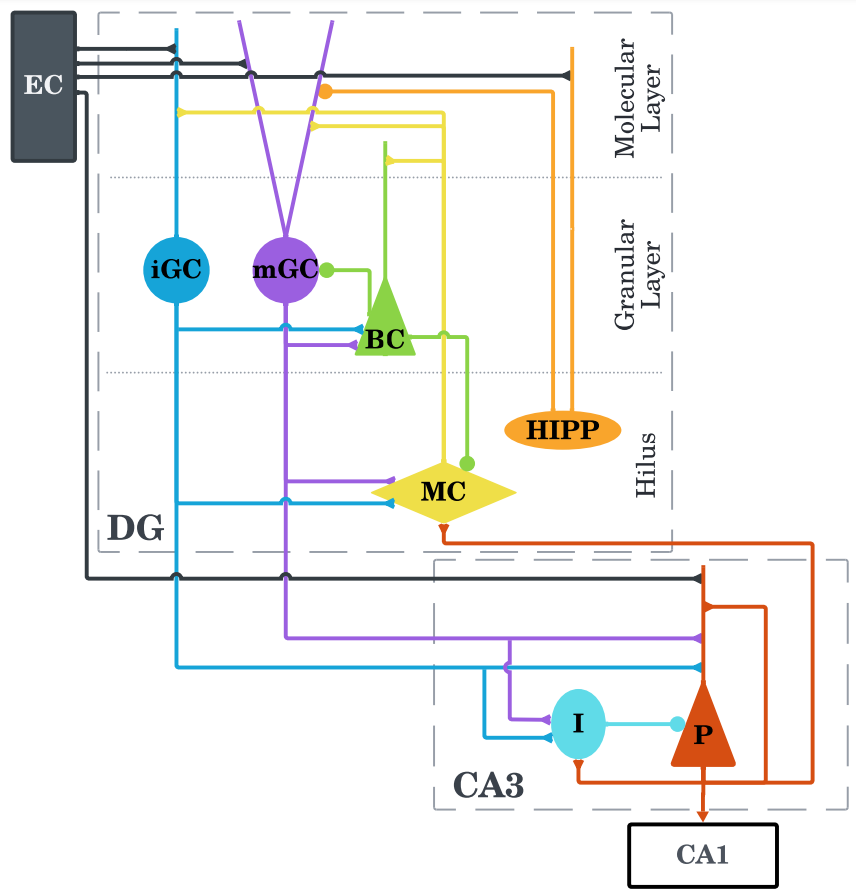
\includegraphics[width=0.9\textwidth]{figuras/arquitetura-rede.png}
    \label{fig:arquitetura-rede}
\end{figure}

A entrada da rede é composta pelas células do córtex entorrinal (EC, \textit{Entorhinal Cortex}), com um total de $N_{EC} = 400$
neurônios~\cite{amaralChapter1990,kimAdult2024}. Em cada simulação, o EC como um todo apresenta um padrão específico, onde cada
padrão é representado por uma subpopulação de 10\% de neurônios do EC ativa~\cite{mcnaughtonDead1991}. Os neurônios inativos não
pertencentes ao padrão não disparam durante a simulação, enquanto que os neurônios ativos disparam de acordo com a distribuição de
Poisson com uma taxa de disparo de $\lambda = \SI{40}{\hertz}$. Os neurônios do EC projetam seus axônios através da via perfurante
para neurônios com dendritos na camada molecular do DG: células granulares (GC, \textit{Granule Cells}), células musgosas (MC,
\textit{Mossy Cells})~\cite{scharfmanHilar2013} e células em cesto (BC, \textit{Basket Cells}); bem como para os neurônios do CA3.

As GCs são subdivididas em duas subpopulações: as células granulares maduras (mGC, \textit{mature Granule Cells}) e as células
granulares imaturas (iGC, \textit{immature Granule Cells}), representando as GCs geradas por neurogênese adulta em sua fase
eletrofisiológica característica de 3-4 semanas de idade~\cite{aimoneRegulation2014}. No total, a rede é composta por $N_{GC} =
2000$ GCs ($\frac{1}{500}$ das $10^6$ células granulares do rato)~\cite{westUnbiased1991}, com 5\% delas sendo
iGCs~\cite{cameronAdult2001}, ou seja $N_{mGC} = 1900$ e $N_{iGC} = 100$. Seguindo a organização lamelar do
DG~\cite{sloviterUpdating2012}, as GCs são distribuídas em 20 lamelas, com 100 células por lamela. Cada GC conecta-se com as BCs,
MCs e neurônios do CA3 da mesma lamela, bem como faz conexões excitatórias aleatórias e não lamelares com as células inibitórias
do hilo associadas à via perfurante (HIPP, \textit{HIlar Perforant Path-associated}).

As BCs ($N_{BC} = 40$) são células inibitórias que garantem a ativação esparsa das GCs através da competição de estilo ``vencedor
leva tudo'' entre elas~\cite{coultripCortical1992,chavlisDendrites2017,kimAdult2024}, onde apenas as GCs mais ativas de uma lamela
se mantêm ativas, inibindo as demais. As HIPPs ($N_{HIPP} = 60$) também contribuem para a esparsidade da ativação das GCs, com uma
inibição mais global, que atua sobre todas as GCs de uma lamela. As MCs ($N_{MC} = 100$) são células excitatórias do hilo que
recebem excitação das GCs e que se projetam para as GCs, BCs e HIPPs através de conexões interlamelares. Por mais que existam
essas projeções excitatórias das MCs para as GCs, seu efeito é, em geral, inibitório através do controle das BCs e
HIPPs~\cite{myersRole2009,scharfmanHilar2013}.

O CA3, diferentemente do DG, não segue uma estrutura lamelar no modelo, já que ele forma uma rede neural muito mais
integrativa~\cite{pakHippocampal2022, watsonHuman2025}. O modelo do CA3 é composto por 600 neurônios piramidais ($N_{PCA3} = 600$)
e 60 neurônios inibitórios ($N_{ICA3} = 60$), modelados de acordo com os dados fisiológicos das células em cesto do
CA3~\cite{wheelerHippocampomeorg2023} de forma a simplificar a variedade de neurônios inibitórios presentes no
CA3~\cite{kopsickFormation2024}. Ambas as populações neuronais recebem aferências do EC e das GCs, com as ICA3s inibindo as PCA3s.
As PCA3s excitam as ICA3s e, importantemente, formam uma rede recorrente ao conectarem-se com outras PCA3s, característica
fundamental para as funções de auto-associação e completamento de padrões do CA3~\cite{kopsickFormation2024,rollsMechanisms2013}.
As PCA3s também enviam retroprojeções para o DG, conectando-se com as MCs no modelo, processo que contribui para a separação de
padrões~\cite{myersPattern2011}.

Todas as simulações foram realizadas com o Brian2~\cite{stimbergBrian2019a}, utilizando o método de Runge-Kutta de 4ª ordem com
passo de tempo fixo de \SI{0.1}{\milli\second}~\cite{butcherHistory1996}.

\section{Modelo de neurônio}

Os neurônios foram modelados de acordo com o modelo de neurônio de Izhikevich de 9
parâmetros~\cite[cap.~8]{izhikevichDynamical2006} e um único compartimento, sem considerar dendritos ou axônios. Esse modelo foi
escolhido por ser capaz de capturar o comportamento dinâmico de neurônios em uma ampla variedade de condições com plausibilidade
biológica, como o modelo de Hodgkin-Huxley~\cite{hodgkinQuantitative1952b}, ao mesmo tempo em que apresenta um modelo matemático
mais simples e computacionalmente mais eficiente. O modelo de neurônio de Izhikevich é descrito pelas seguintes equações:

% (TODO: E por ser a escolha do Hippocampome.org)

\begin{equation}
\label{eq_izhikevich_1}
C_m \frac{dV_m}{dt} = k (V_m - V_r)(V_m - V_t) - u + I
\end{equation}

\begin{equation}
\label{eq_izhikevich_2}
\frac{du}{dt} = a [b(V_m-V_r) - u]
\end{equation}

Onde $V_m$ é o potencial de membrana, $u$ é a variável de recuperação, $C_m$ é a capacitância da membrana, $V_r$ é o
potencial de repouso, $V_t$ é o potencial de limiar, $I$ é a corrente total que flui para o neurônio e $k$, $a$ e $b$ são
constantes que definem as características dinâmicas do neurônio. Além das equações diferenciais acima, que definem a evolução
temporal do potencial de membrana e da variável de recuperação, o modelo de neurônio de Izhikevich também inclui uma regra para
a geração de potenciais de ação, definida pela equação~\ref{eq_izhikevich_3}.

\begin{equation}
\label{eq_izhikevich_3}
\text{se } V_m \geq V_{\text{peak}}, \quad
\begin{cases}
V_m \gets V_{min} \\
u \gets u + d
\end{cases}
\end{equation}

Quando o potencial de membrana atinge o valor de pico $V_{\text{peak}}$, um potencial de ação é gerado e o potencial de membrana é
redefinido para o potencial pós-disparo $V_{min}$ e a variável de recuperação $u$ é incrementada em $d$, dificultando a geração de
um próximo potencial de ação.

% Required packages: \usepackage{amsmath}, \usepackage{graphicx}, \usepackage{multirow}
\begin{table}[h!]
\centering
\renewcommand{\arraystretch}{1.4}
\resizebox{\textwidth}{!}{%
\begin{tabular}{lccccccccc}
\toprule
\multirow{2}{*}{\textbf{Célula}} & \textbf{$k$} & \textbf{$a$} & \textbf{$b$} & \textbf{$d$} & \textbf{$C_m$} & \textbf{$V_r$} & \textbf{$V_t$} & \textbf{$V_{min}$} & \textbf{$V_{peak}$} \\
 & (nS/mV) & (ms$^{-1}$) & (nS) & (pA) & (pF) & (mV) & (mV) & (mV) & (mV) \\
\midrule
$\vcenter{\hbox{
\includegraphics[height=1.5em]{figuras/neurônios/mgc.png}}}$ Granular madura & 0.45 & 0.003 & 24.48 & 50 & 38 & -77.4 & -44.9 & -66.47 & 15.49 \\
$\vcenter{\hbox{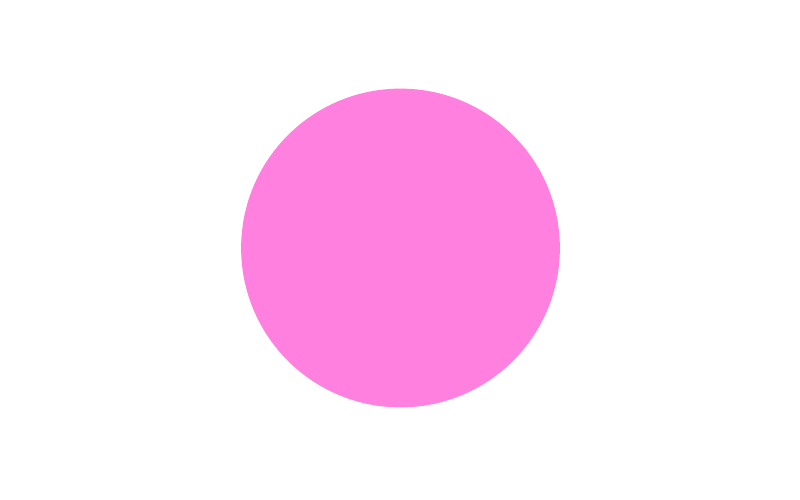
\includegraphics[height=1.5em]{figuras/neurônios/igc.png}}}$ Granular imatura & 0.139 & 0.002 & -1.877 & 12.149 & 24.6 & -63.66 & -38.41 & -48.2 & 83.5 \\
$\vcenter{\hbox{
\includegraphics[height=1.5em]{figuras/neurônios/mc.png}}}$ Musgosa & 1.5 & 0.004 & -20.84 & 117 & 258 & -63.67 & -37.11 & -47.98 & 28.29 \\
$\vcenter{\hbox{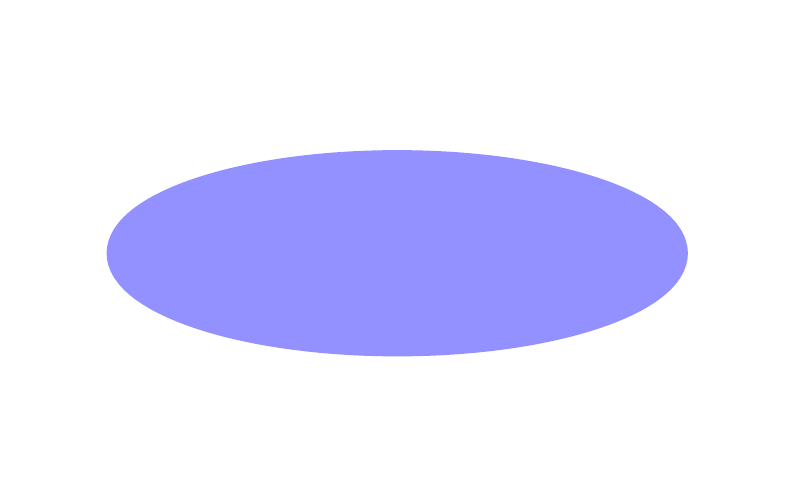
\includegraphics[height=1.5em]{figuras/neurônios/hipp.png}}}$ HIPP & 0.01 & 0.004 & -2 & 40.52 & 58.7 & -70 & -50 & -75 & 90 \\
$\vcenter{\hbox{
\includegraphics[height=1.5em]{figuras/neurônios/bc.png}}}$ Em cesto & 0.81 & 0.097 & 1.89 & 553 & 208 & -61.02 & -37.84 & -36.23 & 14.08 \\
$\vcenter{\hbox{
\includegraphics[height=1.5em]{figuras/neurônios/pca3.png}}}$ Piramidal do CA3 & 0.79 & 0.008 & -42.55 & 588 & 366 & -63.2 & -33.6 & -38.87 & 35.86 \\
$\vcenter{\hbox{
\includegraphics[height=1.5em]{figuras/neurônios/ica3.png}}}$ Inibitória do CA3 & 1 & 0.004 & 9.26 & -6 & 45 & -57.51 & -23.38 & -47.56 & 18.45 \\
\bottomrule
\end{tabular}}
\caption{Parâmetros do modelo Izhikevich por tipo de neurônio.}\label{tab:izhikevich_neuron_params}
\end{table}


\section{Modelo de sinapse}

O modelo de sinapse, assim como o de neurônio, foi definido a partir do Hippocampome.org~\cite{wheelerHippocampomeorg2023},
seguindo a formulação de~\citeonline{sennAlgorithm2001,mongilloSynaptic2008a}. Esse modelo modela a
plasticidade de curto prazo, seja ela depressão de curto prazo, causada pela depleção de neurotransmissores, ou potenciação de
curto prazo, causada pelo acúmulo de cálcio, ambas na escala dos décimos de segundos. Cada sinapse possui 5 parâmetros (descritos
na Tabela~\ref{tab:synapse_params}): a condutância máxima da sinapse no caso de nenhuma depleção de recursos sinápticos $g$, a proporção de
recursos utilizados a cada disparo $U_{se}$, a constante de tempo de decaimento da corrente sináptica $\tau_d$,
a constante de tempo de facilitação $\tau_f$, e a constante de tempo de recuperação dos recursos $\tau_r$~\cite{moradiNormalized2022}.

O modelo é descrito por três variáveis de estado: a utilização dos recursos sinápticos ($U$), a recuperação desses recursos ($R$)
e a porcentagem de recursos em estado ativo ($A$). Inicialmente, $U_{t_0} = 0$, $R_{t_0} = 1$ e $A_{t_0} = 0$, 
visto que todos os recursos estão disponíveis para ser utilizados. A evolução temporal dessas
variáveis é governada pelo seguinte sistema de equações diferenciais:

\begin{equation}
    \label{eq_tsodyks_dU}
    \frac{dU}{dt} = \frac{-U}{\tau_f} + U_{se}(1-U_{-}) \delta(\Delta t_i)
\end{equation}

\begin{equation}
    \label{eq_tsodyks_dR}
    \frac{dR}{dt} = \frac{1-R-A}{\tau_r} - U_{+} R_{-} \delta(\Delta t_i)
\end{equation}

\begin{equation}
    \label{eq_tsodyks_dA}
    \frac{dA}{dt} = \frac{-A}{\tau_d} + U_{+} R_{-} \delta(\Delta t_i)
\end{equation}

nde $\delta$ é a função delta de Dirac, que resulta em 1 apenas quando $\Delta t_i = t - t_i = 0$, ou seja, apenas no tempo $t$
correspondente ao tempo do evento sináptico $t_i$. $U_{+}$ corresponde ao valor de $U$ logo após o evento sináptico, enquanto que
$R_{-}$ corresponde ao valor de $R$ logo antes do mesmo.

A partir dessas equações, a corrente sináptica é dada por:

\begin{equation}
    \label{eq_tsodyks_I}
    I = k \cdot A \cdot g \cdot (V_m - E)
\end{equation}

onde $V_m$ é o potencial de membrana do neurônio pós-sináptico, $E$ é o potencial de reversão da sinapse, para sinapses
inibitórias e excitatórias, respectivamente, $E_{inh} = \SI{-86}{\milli\volt}$ e $E_{exc} = \SI{0}{\milli\volt}$, e $k$
é uma constante de escala definida como $k = 10$ para todas as sinapses. Essa constante de escala é necessária por conta
da escala reduzida da rede, visto que, pelo baixo número de sinapses do modelo comparado ao hipocampo do rato, sem o 
escalamento a rede toda ficaria silenciosa.


% Synapse Parameters Table
% Required packages: \usepackage{amsmath}, \usepackage{graphicx}, \usepackage{multirow}
\begin{table}[h!]
\centering
\renewcommand{\arraystretch}{1.4}
\resizebox{\textwidth}{!}{%
\begin{tabular}{llccccccc}
\toprule
\multirow{2}{*}{\textbf{Pré-sináptico}} & \multirow{2}{*}{\textbf{Pós-sináptico}} & \multirow{2}{*}{\textbf{Conexão}} & $P$ & \textbf{$g$} & \textbf{$\tau_d$} & \textbf{$\tau_r$} & \textbf{$\tau_f$} & \textbf{$U$} \\
 & & & (\%) & (nS) & (ms) & (ms) & (ms) &  \\
\midrule
$\vcenter{\hbox{
\includegraphics[height=1.5em]{figuras/neurônios/pp.png}}}$ Córtex Entorrinal & $\vcenter{\hbox{
\includegraphics[height=1.5em]{figuras/neurônios/mgc.png}}}$ Granular madura & Aleatória & 8 & 1.825 & 5.333 & 266.239 & 18.714 & 0.27 \\
$\vcenter{\hbox{
\includegraphics[height=1.5em]{figuras/neurônios/pp.png}}}$ Córtex Entorrinal & $\vcenter{\hbox{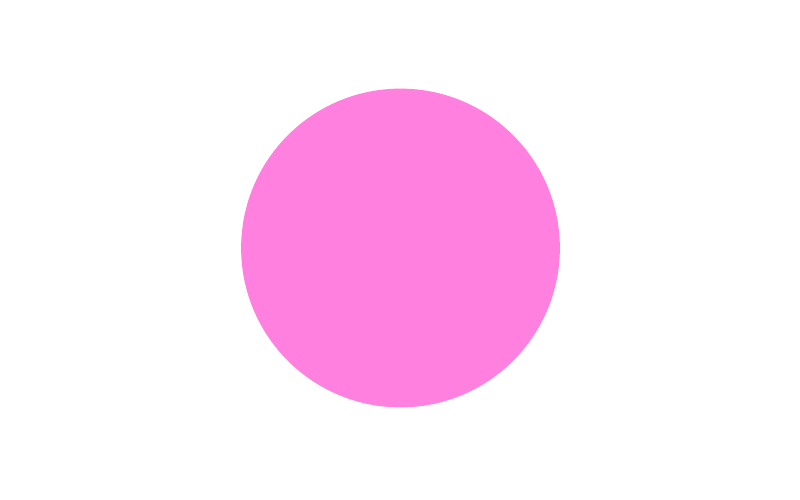
\includegraphics[height=1.5em]{figuras/neurônios/igc.png}}}$ Granular imatura & Aleatória & 8 & 1.825 & 5.333 & 266.239 & 18.714 & 0.27 \\
$\vcenter{\hbox{
\includegraphics[height=1.5em]{figuras/neurônios/pp.png}}}$ Córtex Entorrinal & $\vcenter{\hbox{
\includegraphics[height=1.5em]{figuras/neurônios/mc.png}}}$ Musgosa & Aleatória & 20 & 1.422 & 4.671 & 319.835 & 57.766 & 0.204 \\
$\vcenter{\hbox{
\includegraphics[height=1.5em]{figuras/neurônios/pp.png}}}$ Córtex Entorrinal & $\vcenter{\hbox{
\includegraphics[height=1.5em]{figuras/neurônios/bc.png}}}$ Em cesto & Aleatória & 20 & 1.406 & 3.849 & 144.415 & 48.2 & 0.214 \\
$\vcenter{\hbox{
\includegraphics[height=1.5em]{figuras/neurônios/pp.png}}}$ Córtex Entorrinal & $\vcenter{\hbox{
\includegraphics[height=1.5em]{figuras/neurônios/pca3.png}}}$ Piramidal do CA3 & Aleatória & 4 & 1.065 & 6.55 & 258.318 & 53.478 & 0.184 \\
$\vcenter{\hbox{
\includegraphics[height=1.5em]{figuras/neurônios/pp.png}}}$ Córtex Entorrinal & $\vcenter{\hbox{
\includegraphics[height=1.5em]{figuras/neurônios/ica3.png}}}$ Inibitória do CA3 & Aleatória & 20 & 1.556 & 3.602 & 457.468 & 35.904 & 0.21 \\
$\vcenter{\hbox{
\includegraphics[height=1.5em]{figuras/neurônios/mgc.png}}}$ Granular madura & $\vcenter{\hbox{
\includegraphics[height=1.5em]{figuras/neurônios/mc.png}}}$ Musgosa & Lamelar & 20 & 1.713 & 5.347 & 428.583 & 73.479 & 0.151 \\
$\vcenter{\hbox{
\includegraphics[height=1.5em]{figuras/neurônios/mgc.png}}}$ Granular madura & $\vcenter{\hbox{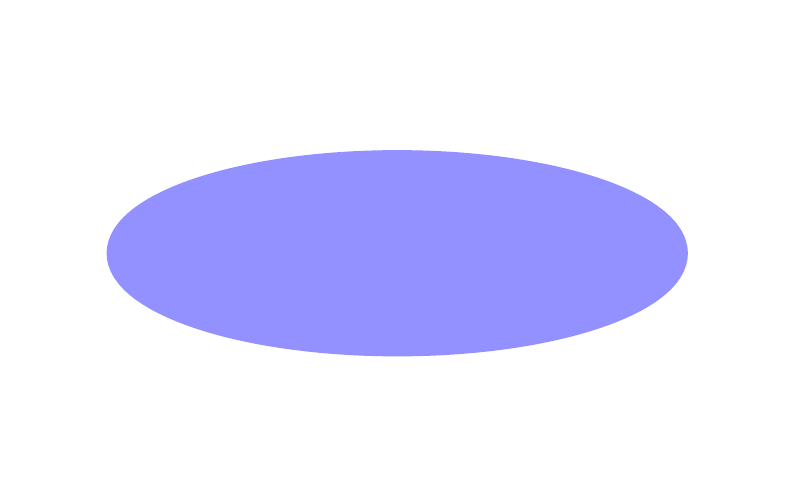
\includegraphics[height=1.5em]{figuras/neurônios/hipp.png}}}$ HIPP & Aleatória & 5 & 1.305 & 5.181 & 462.814 & 48.986 & 0.15 \\
$\vcenter{\hbox{
\includegraphics[height=1.5em]{figuras/neurônios/mgc.png}}}$ Granular madura & $\vcenter{\hbox{
\includegraphics[height=1.5em]{figuras/neurônios/bc.png}}}$ Em cesto & Lamelar & 100 & 1.458 & 3.566 & 151.265 & 62.278 & 0.197 \\
$\vcenter{\hbox{
\includegraphics[height=1.5em]{figuras/neurônios/mgc.png}}}$ Granular madura & $\vcenter{\hbox{
\includegraphics[height=1.5em]{figuras/neurônios/pca3.png}}}$ Piramidal do CA3 & Lamelar & 60 & 1.384 & 6.657 & 278.286 & 78.584 & 0.155 \\
$\vcenter{\hbox{
\includegraphics[height=1.5em]{figuras/neurônios/mgc.png}}}$ Granular madura & $\vcenter{\hbox{
\includegraphics[height=1.5em]{figuras/neurônios/ica3.png}}}$ Inibitória do CA3 & Lamelar & 100 & 1.625 & 3.915 & 518.934 & 43.274 & 0.176 \\
$\vcenter{\hbox{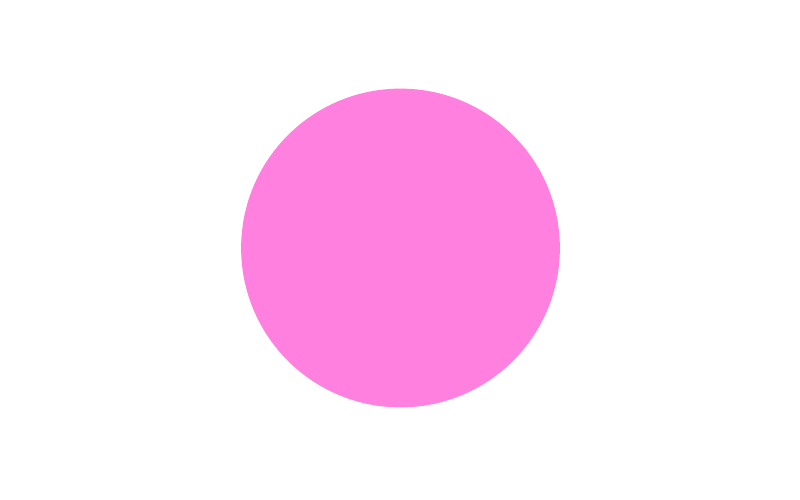
\includegraphics[height=1.5em]{figuras/neurônios/igc.png}}}$ Granular imatura & $\vcenter{\hbox{
\includegraphics[height=1.5em]{figuras/neurônios/mc.png}}}$ Musgosa & Lamelar & 20 & 1.713 & 5.347 & 428.583 & 73.479 & 0.151 \\
$\vcenter{\hbox{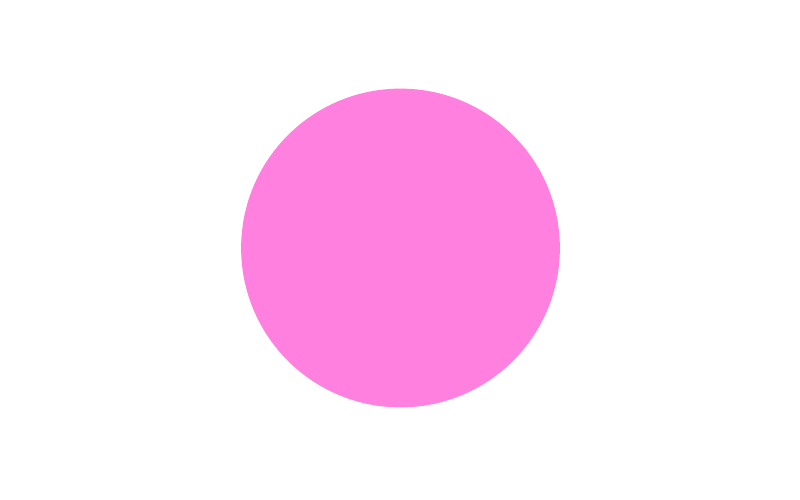
\includegraphics[height=1.5em]{figuras/neurônios/igc.png}}}$ Granular imatura & $\vcenter{\hbox{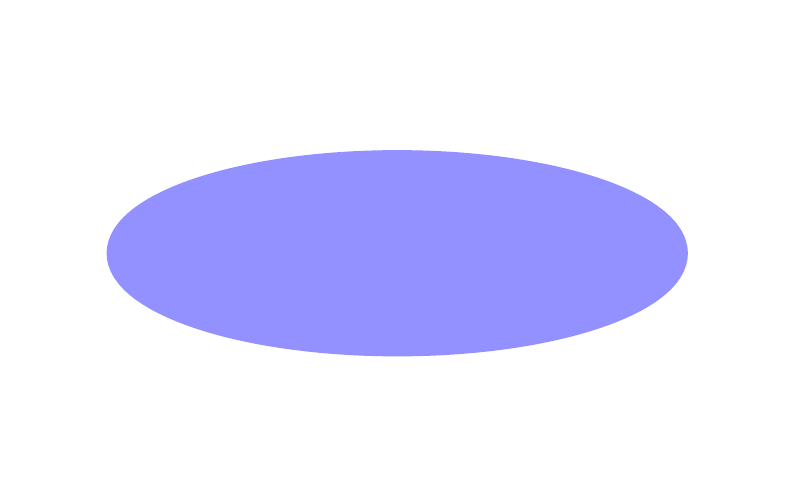
\includegraphics[height=1.5em]{figuras/neurônios/hipp.png}}}$ HIPP & Aleatória & 5 & 1.305 & 5.181 & 462.814 & 48.986 & 0.15 \\
$\vcenter{\hbox{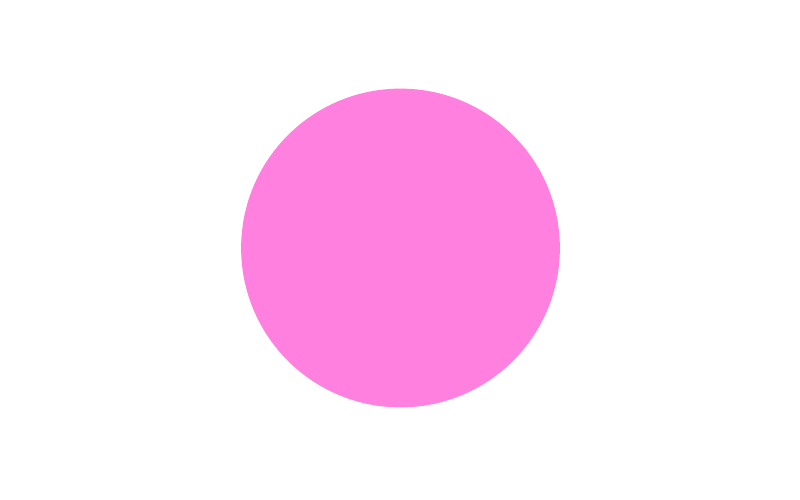
\includegraphics[height=1.5em]{figuras/neurônios/igc.png}}}$ Granular imatura & $\vcenter{\hbox{
\includegraphics[height=1.5em]{figuras/neurônios/bc.png}}}$ Em cesto & Lamelar & 100 & 1.458 & 3.566 & 151.265 & 62.278 & 0.197 \\
$\vcenter{\hbox{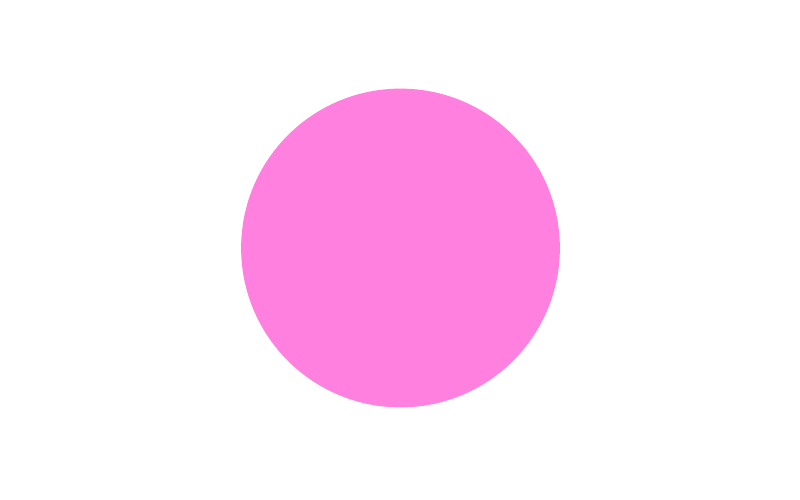
\includegraphics[height=1.5em]{figuras/neurônios/igc.png}}}$ Granular imatura & $\vcenter{\hbox{
\includegraphics[height=1.5em]{figuras/neurônios/pca3.png}}}$ Piramidal do CA3 & Lamelar & 60 & 1.384 & 6.657 & 278.286 & 78.584 & 0.155 \\
$\vcenter{\hbox{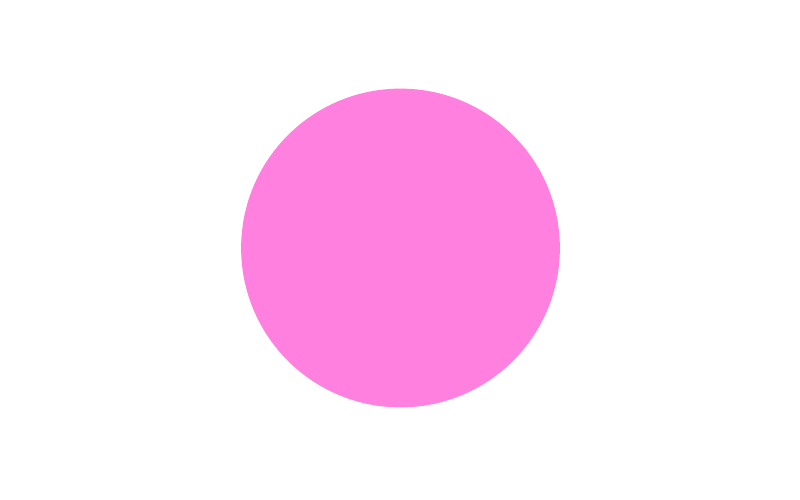
\includegraphics[height=1.5em]{figuras/neurônios/igc.png}}}$ Granular imatura & $\vcenter{\hbox{
\includegraphics[height=1.5em]{figuras/neurônios/ica3.png}}}$ Inibitória do CA3 & Lamelar & 100 & 1.625 & 3.915 & 518.934 & 43.274 & 0.176 \\
$\vcenter{\hbox{
\includegraphics[height=1.5em]{figuras/neurônios/mc.png}}}$ Musgosa & $\vcenter{\hbox{
\includegraphics[height=1.5em]{figuras/neurônios/mgc.png}}}$ Granular madura & Interlamelar & 0.2 & 2.394 & 5.357 & 166.162 & 20.224 & 0.304 \\
$\vcenter{\hbox{
\includegraphics[height=1.5em]{figuras/neurônios/mc.png}}}$ Musgosa & $\vcenter{\hbox{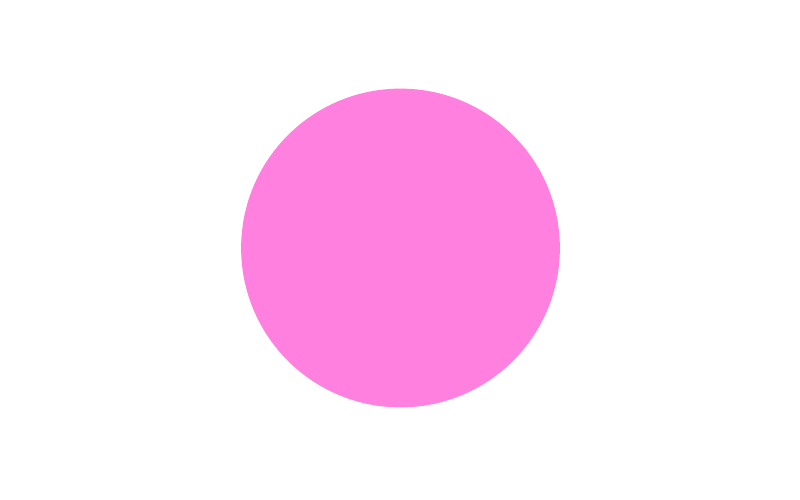
\includegraphics[height=1.5em]{figuras/neurônios/igc.png}}}$ Granular imatura & Interlamelar & 0.2 & 2.394 & 5.357 & 166.162 & 20.224 & 0.304 \\
$\vcenter{\hbox{
\includegraphics[height=1.5em]{figuras/neurônios/mc.png}}}$ Musgosa & $\vcenter{\hbox{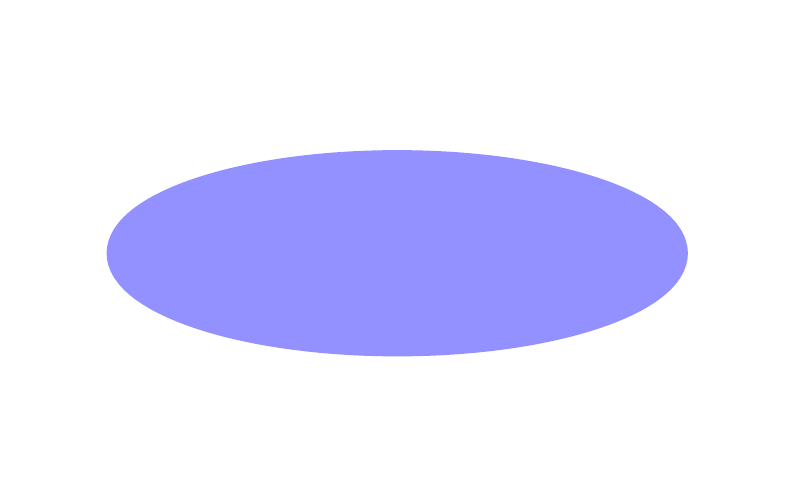
\includegraphics[height=1.5em]{figuras/neurônios/hipp.png}}}$ HIPP & Interlamelar & 100 & 1.376 & 4.824 & 358.431 & 54.872 & 0.181 \\
$\vcenter{\hbox{
\includegraphics[height=1.5em]{figuras/neurônios/mc.png}}}$ Musgosa & $\vcenter{\hbox{
\includegraphics[height=1.5em]{figuras/neurônios/bc.png}}}$ Em cesto & Interlamelar & 100 & 1.996 & 3.396 & 117.365 & 69.316 & 0.255 \\
$\vcenter{\hbox{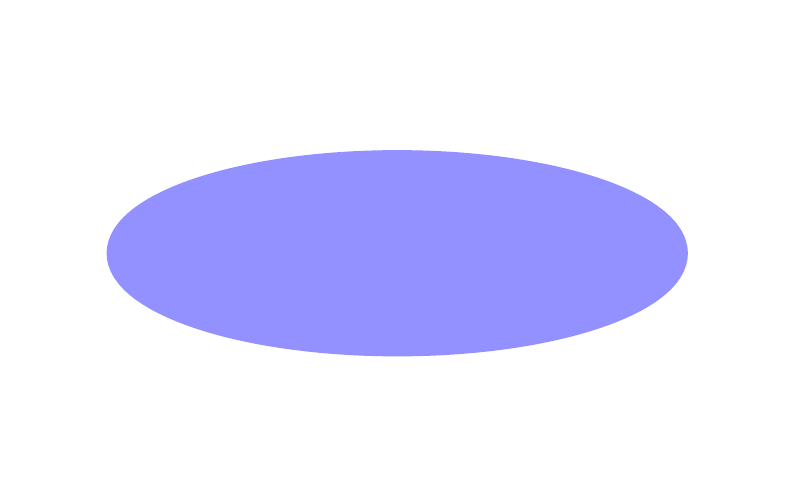
\includegraphics[height=1.5em]{figuras/neurônios/hipp.png}}}$ HIPP & $\vcenter{\hbox{\includegraphics[height=1.5em]{figuras/neurônios/mgc.png}}}$ Granular madura & Aleatória & 20 & 2.002 & 8.935 & 559.143 & 8.396 & 0.278 \\
$\vcenter{\hbox{\includegraphics[height=1.5em]{figuras/neurônios/hipp.png}}}$ HIPP & $\vcenter{\hbox{\includegraphics[height=1.5em]{figuras/neurônios/igc.png}}}$ Granular imatura & Aleatória & 10 & 2.002 & 8.935 & 559.143 & 8.396 & 0.278 \\
$\vcenter{\hbox{\includegraphics[height=1.5em]{figuras/neurônios/hipp.png}}}$ HIPP & $\vcenter{\hbox{\includegraphics[height=1.5em]{figuras/neurônios/bc.png}}}$ Em cesto & Aleatória & 2 & 1.709 & 5.982 & 367.198 & 15.292 & 0.221 \\
$\vcenter{\hbox{\includegraphics[height=1.5em]{figuras/neurônios/bc.png}}}$ Em cesto & $\vcenter{\hbox{\includegraphics[height=1.5em]{figuras/neurônios/mgc.png}}}$ Granular madura & Lamelar & 100 & 2.451 & 6.543 & 433.876 & 6.347 & 0.332 \\
$\vcenter{\hbox{\includegraphics[height=1.5em]{figuras/neurônios/bc.png}}}$ Em cesto & $\vcenter{\hbox{\includegraphics[height=1.5em]{figuras/neurônios/igc.png}}}$ Granular imatura & Lamelar & 100 & 2.451 & 6.543 & 433.876 & 6.347 & 0.332 \\
$\vcenter{\hbox{\includegraphics[height=1.5em]{figuras/neurônios/bc.png}}}$ Em cesto & $\vcenter{\hbox{\includegraphics[height=1.5em]{figuras/neurônios/hipp.png}}}$ HIPP & Aleatória & 2 & 1.408 & 6.544 & 534.182 & 8.385 & 0.24 \\
$\vcenter{\hbox{\includegraphics[height=1.5em]{figuras/neurônios/pca3.png}}}$ Piramidal do CA3 & $\vcenter{\hbox{\includegraphics[height=1.5em]{figuras/neurônios/pca3.png}}}$ Piramidal do CA3 & Aleatória & 2 & 0.603 & 9.516 & 278.258 & 27.513 & 0.172 \\
$\vcenter{\hbox{\includegraphics[height=1.5em]{figuras/neurônios/pca3.png}}}$ Piramidal do CA3 & $\vcenter{\hbox{\includegraphics[height=1.5em]{figuras/neurônios/mc.png}}}$ Musgosa & Lamelar & 10 & 2.035 & 4.297 & 359.116 & 40.457 & 0.236 \\
$\vcenter{\hbox{\includegraphics[height=1.5em]{figuras/neurônios/pca3.png}}}$ Piramidal do CA3 & $\vcenter{\hbox{\includegraphics[height=1.5em]{figuras/neurônios/ica3.png}}}$ Inibitória do CA3 & Aleatória & 100 & 1.247 & 4.525 & 525.605 & 23.321 & 0.189 \\
$\vcenter{\hbox{\includegraphics[height=1.5em]{figuras/neurônios/ica3.png}}}$ Inibitória do CA3 & $\vcenter{\hbox{\includegraphics[height=1.5em]{figuras/neurônios/pca3.png}}}$ Piramidal do CA3 & Aleatória & 100 & 1.462 & 7.793 & 416.282 & 20.63 & 0.203 \\
\bottomrule
\end{tabular}}
\caption{Parâmetros das sinapses entre as populações neuronais. Conexões aleatórias ocorrem entre todas as células
              de ambas as populações; conexões lamelares ocorrem entre células da mesma lamela; conexões interlamelares ocorrem
              entre as células de uma lamela com todas as demais. A probabilidade de conexão $P$ diz respeito à porcentagem de
              conexões entre as populações neuronais de acordo com a condição de conexão.}
\label{tab:synapse_params}
\end{table}



\section{Plasticidade de longo prazo}

\section{Neurogênese temporal}

\section{Separação de padrões}

A metodologia para quantificar a separação de padrões foi baseada na que foi utilizada em~\cite{kimEffect2024}.
Para caracterizar a separação de padrões, é comparada a sobreposição entre os padrões de atividade neural na entrada (células do
córtex entorrinal) e na saída (células granulares do DG, ou piramidais do CA3) da rede. Um padrão é definido por um
representação binária de tamanho $N$, onde $N$ é o número total de neurônios de uma população específica, em que neurônios que
dispararam ao menos uma vez durante o intervalo de tempo da simulação são representados por 1 e os que não dispararam são
representados por 0. Para um par de padrões $A^{(l)}$ e $B^{(l)}$ (onde $l \in \{in, out\}$ para entrada e saída,
respectivamente), a distância entre os padrões $D_p^{(l)}$ é definida como:

\begin{equation}
    \label{eq:dp}
    D_p^{(l)} = \frac{O^{(l)}}{D_a^{(l)}}
\end{equation}

Nesta equação, $O^{(l)}$ representa o grau de ortogonalização e $D_a^{(l)}$ o grau médio de ativação dos dois padrões. O grau médio de ativação $D_a^{(l)}$ é a média aritmética dos graus de ativação de cada padrão, $A^{(l)}$ e $B^{(l)}$:

\begin{equation}
    \label{eq:da}
    D_a^{(l)} = \frac{D_a^{(A^{(l)})} + D_a^{(B^{(l)})}}{2}
\end{equation}

O grau de ativação de um padrão individual é a fração de neurônios ativos (representados por 1 em uma codificação binária) no padrão.
O grau de ortogonalização $O^{(l)}$, que mede a dissimilaridade entre os padrões, é calculado a partir do coeficiente de correlação de Pearson, $\rho^{(l)}$:

\begin{equation}
    \label{eq:o}
    O^{(l)} = \frac{1 - \rho^{(l)}}{2}
\end{equation}

Onde $\rho^{(l)}$ é o coeficiente de correlação de Pearson entre os padrões $A^{(l)}$ e $B^{(l)}$.
Considerando $\{a_i^{(l)}\}$ e $\{b_i^{(l)}\}$ ($i=1, \dots, N_l$) como as representações binárias do estado da $i$-ésima célula nos padrões $A^{(l)}$ e $B^{(l)}$ ($l \in \{in, out\}$), o coeficiente de correlação de Pearson é dado por:

\begin{equation}
    \label{eq:pearson}
    \rho^{(l)} = \frac{\sum_{i=1}^{N_l} \Delta a_i^{(l)} \cdot \Delta b_i^{(l)}}{\sqrt{\sum_{i=1}^{N_l} (\Delta a_i^{(l)})^2} \sqrt{\sum_{i=1}^{N_l} (\Delta b_i^{(l)})^2}}
\end{equation}

em que $\Delta a_i^{(l)} = a_i^{(l)} - \langle a^{(l)} \rangle$ e $\Delta b_i^{(l)} = b_i^{(l)} - \langle b^{(l)} \rangle$. A notação $\langle \dots \rangle$ indica a média populacional sobre todas as células. O valor de $\rho^{(l)}$ varia entre -1 e 1.
A similaridade entre os padrões, $C^{(l)}$, é diretamente o coeficiente de correlação de Pearson:

\begin{equation}
    \label{eq:c}
    C^{(l)} = \rho^{(l)}
\end{equation}

A partir das distâncias dos padrões de entrada ($D_p^{(in)}$) e saída ($D_p^{(out)}$), o grau de separação de padrões, $S_d$, é calculado como a razão entre elas:

\begin{equation}
    \label{eq:sd}
    S_d = \frac{D_p^{(out)}}{D_p^{(in)}}
\end{equation}

Um valor de $S_d > 1$ indica que os padrões de saída são mais distintos que os de entrada, caracterizando a separação de padrões. Inversamente, $S_d < 1$ indica uma convergência de padrões, onde os padrões de saída se tornam mais similares entre si.





\chapter{Resultados}

\section{Separação de padrões}


Alguns resultados iniciais a partir do protocolo descrito na Seção~\ref{sec:separacao_padroes} já foram obtidos e serão discutidos
nesta seção.

A Figura~\ref{fig:avg_activity} apresenta a ativação média das populações de GCs para o modelo de controle (sem neurogênese) e
para os modelos com neurogênese em diferentes níveis de conectividade das iGCs com o CE. No modelo de controle, onde todas as GCs
são maduras, a ativação média da população, definida pela porcentagem de células que dispararam ao menos uma vez durante o
intervalo de \SI{1000}{\milli\second} da simulação, foi de 12.46\%, um nível de ativação esparsa, mas não tão baixo quanto o
observado no DG. Em simulações futuras, será analisado o impacto de um aumento de sinapses inibitórias no circuito.

A introdução de iGCs no circuito altera significativamente essa dinâmica. Conforme a conectividade das iGCs aumenta, a sua taxa de
ativação cresce acentuadamente, o que é consistente com sua maior excitabilidade intrínseca. No cenário de 100\% de conectividade,
praticamente toda a população de iGCs se torna ativa em resposta a um padrão de entrada. Esse aumento na atividade das iGCs eleva
a ativação geral da população de GCs.

Em contrapartida, observa-se uma diminuição progressiva na atividade das GCs maduras (mGCs) à medida que a conectividade das iGCs
aumenta. Este resultado sugere a existência de um mecanismo de competição inibitória, onde as iGCs, ao serem fortemente ativadas,
acabam por suprimir indiretamente a atividade das mGCs através dos interneurônios compartilhados.

Contudo, a supressão observada nas mGCs não é tão acentuada quanto a reportada em outros modelos~\cite{kimEffect2024}, o que pode
indicar novamente que a força da inibição no modelo atual seja insuficiente. Uma hipótese para essa discrepância é a ausência de
uma via inibitória direta das iGCs para as mGCs, um mecanismo descrito por~\citeonline{lunaAdultborn2019} que não foi
implementado. A inclusão dessa conexão direta é uma via promissora para futuras investigações, podendo conferir maior realismo
biológico ao modelo e também será explorada no projeto.

\begin{figure}[H]
    \centering
    \caption{Ativação média da população (\%) por modelo. O eixo vertical possui uma descontinuidade e duas escalas diferentes para melhor visualização. O erro é representado pela área sombreada.}
    \includegraphics[width=0.7\textwidth]{figuras/plots/avg_activity}
    \label{fig:avg_activity}
\end{figure}


A Figura~\ref{fig:pattern_separation} aprofunda a análise ao detalhar o grau de separação de padrões ($\mathcal{S}_D$) em função
da similaridade dos padrões de entrada. Um valor de $\mathcal{S}_D > 1$ significa que a representação de saída no DG é mais
distinta do que a representação de entrada no CE. De forma geral, observa-se que todos os modelos, incluindo o de controle,
alcançam uma separação de padrões mais elevada para entradas altamente similares. Isso ocorre porque, matematicamente, pequenas
diferenças na codificação de saída são amplificadas quando a sobreposição na entrada é muito grande. O desempenho do modelo de
controle com entradas de baixa similaridade foi subótimo, não conseguindo separar os padrões de forma eficaz, o que pode ser
novamente atribuído à esparsidade insuficiente da rede, como discutido anteriormente. A introdução da neurogênese exacerba essa
limitação: à medida que a conectividade das iGCs aumenta, a capacidade de separação de padrões da rede diminui progressivamente. O
modelo com 100\% de conectividade das iGCs apresenta o pior desempenho em todas as condições de similaridade. O mecanismo
subjacente a essa deterioração é a ativação promíscua das iGCs, que, devido à sua alta excitabilidade, tendem a formar um mesmo
subconjunto de neurônios ativos em resposta a padrões de entrada distintos, reduzindo a dissimilaridade das representações na
saída e, consequentemente, o grau de separação de padrões.

\begin{figure}
    \centering
    \caption{Grau de separação de padrões ($\mathcal{S}_D$) por modelo e nível de similaridade de entrada. A linha tracejada
    representa um grau de separação de 1, valores acima disso indicam que houve separação de padrões, enquanto que valores abaixo
    disso indicam que não houve separação. O erro é representado pela área sombreada.}
    \includegraphics[width=0.7\textwidth]{figuras/plots/pattern_separation}
    \label{fig:pattern_separation}
\end{figure}

Para dissecar as contribuições individuais de cada população neuronal, a Figura~\ref{fig:avg_pattern_separation} apresenta o
$\mathcal{S}_D$ médio, agregado sobre todos os níveis de similaridade. Esta análise confirma a tendência observada anteriormente,
mostrando que a capacidade de separação de padrões do conjunto total de GCs diminui com o aumento da conectividade das iGCs. A
análise das subpopulações revela uma clara dicotomia funcional: as iGCs, isoladamente, nunca alcançam um $\mathcal{S}_D > 1$,
indicando que, em vez de separar, elas integram os padrões de entrada, tornando-os mais similares. Em contraste, as mGCs
demonstram uma robusta capacidade de separação de padrões em todos os modelos. 

O desempenho das mGCs melhora ligeiramente com o aumento da conectividade e atividade das iGCs, provavelmente um subproduto do
aumento da inibição global na rede, que, embora insuficiente, pode estar tornando a atividade das mGCs marginalmente mais esparsa.
Um modelo de regressão linear simples foi utilizado para avaliar a relação entre o nível de conectividade das iGCs e o grau de
separação de padrões das mGCs. O modelo encontrou uma relação significativa, embora fraca, entre o nível de conectividade e o grau
de separação de padrões ($F(1, 8) = 7.83, p = 0.023, R^2 = 0.49, \mathcal{S}^{mGC}_D = 1.76 + 0.13 \times \text{Conectividade}$).

Esses achados corroboram a teoria proposta por~\citeonline{kimEffect2024}, que sugere um papel das mGCs como separadoras de
padrões e das iGCs como integradoras. Resta investigar, em experimentos futuros, qual o impacto dessa codificação mista e do
fortalecimento da separação nas mGCs para as funções de memória no CA3.

\begin{figure}
    \centering
    \caption{Grau de separação de padrões ($\mathcal{S}_D$) médio por modelo e população. A linha tracejada em preto representa o
    $\mathcal{S}_D$ do controle, enquanto que a em cinza representa um grau de separação de 1. O erro é representado pela área
    sombreada; neste caso, o erro é muito grande, visto que o $\mathcal{S}_D$ varia muito entre diferentes níveis de similaridade
    na Figura~\ref{fig:pattern_separation}.}
    \includegraphics[width=0.7\textwidth]{figuras/plots/avg_pattern_separation}
    \label{fig:avg_pattern_separation}
\end{figure}


\section{Resultados esperados}

Espera-se que a presença de iGCs prejudique o completamento de padrões no CA3, devido a uma maior ativação de assembleias
neuronais não relacionadas ao padrão de entrada, um efeito consistente com resultados experimentais que sugerem uma ativação
promíscua de assembleias por parte das iGCs devido à sua alta excitabilidade~\cite{koSystems2025}. Adicionalmente, na simulação da
maturação temporal, espera-se que as iGCs passem a codificar os padrões no tempo, integrando informações que foram apresentadas
enquanto eram jovens, corroborando seu papel como integradoras temporais, como proposto por~\cite{aimoneComputational2009}.
Teoriza-se, portanto, que as mGCs teriam um papel predominante na separação de padrões específicos e distintos, enquanto as iGCs,
ao longo de sua maturação, se especializariam na separação de padrões próximos no tempo, ou seja, aqueles que codificaram durante
sua fase imatura.

\chapter{Cronograma}

\definecolor{v}{HTML}{A4C6A4}
\definecolor{x}{HTML}{808080}
\definecolor{b}{HTML}{FFFFFF}

\newcommand{\rowlabel}[1]{\parbox[c][3.2cm][c]{4.5cm}{\centering\textbf{#1}}}
\newcommand{\firstcolcell}[1]{\parbox[c][1.6cm][c]{4.5cm}{\raggedright #1}}

\begin{table}[H]
    \centering
    \caption{Cronograma de atividades}
    \begin{tabularx}{\textwidth}{|p{4.5cm}|*{8}{>{\centering\arraybackslash}X|}}
        \hline
        \multirow{2}{*}{} & \multicolumn{8}{c|}{\textbf{Trimestre}} \\
        \cline{2-9}
        & \textbf{1} & \textbf{2} & \textbf{3} & \textbf{4} & \textbf{5} & \textbf{6} & \textbf{7} & \textbf{8} \\
        \hline
        \firstcolcell{Revisão de literatura}
        & \cellcolor{v} & \cellcolor{v} & \cellcolor{v} & \cellcolor{v} & \cellcolor{x} & \cellcolor{x} & \cellcolor{x} & \cellcolor{b} \\
        \hline
        \firstcolcell{Implementação do modelo do DG}
        & \cellcolor{v} & \cellcolor{v} & \cellcolor{v} & \cellcolor{v} & \cellcolor{b} & \cellcolor{b} & \cellcolor{b} & \cellcolor{b} \\
        \hline
        \firstcolcell{Implementação do modelo do CA3}
        & \cellcolor{b} & \cellcolor{v} & \cellcolor{v} & \cellcolor{v} & \cellcolor{x} & \cellcolor{x} & \cellcolor{b} & \cellcolor{b} \\
        \hline
        \firstcolcell{Escrita da dissertação}
        & \cellcolor{b} & \cellcolor{b} & \cellcolor{v} & \cellcolor{v} & \cellcolor{x} & \cellcolor{x} & \cellcolor{x} & \cellcolor{x} \\
        \hline
        \firstcolcell{Análise da separação de padrões}
        & \cellcolor{b} & \cellcolor{b} & \cellcolor{b} & \cellcolor{v} & \cellcolor{b} & \cellcolor{b} & \cellcolor{x} & \cellcolor{b} \\
        \hline
        \firstcolcell{Implementação da maturação temporal}
        & \cellcolor{b} & \cellcolor{b} & \cellcolor{b} & \cellcolor{b} & \cellcolor{x} & \cellcolor{x} & \cellcolor{x} & \cellcolor{b} \\
        \hline
        \firstcolcell{Análise da auto-associação e completamento de padrões}
        & \cellcolor{b} & \cellcolor{b} & \cellcolor{b} & \cellcolor{b} & \cellcolor{b} & \cellcolor{b} & \cellcolor{x} & \cellcolor{x} \\
        \hline
    \end{tabularx}
    \label{tab:cronograma}
    \vspace{1em}
    \par
    \noindent \colorbox{v}{\phantom{XX}} \hspace{1ex} Feito
    \hspace{2em}
    \colorbox{x}{\phantom{XX}} \hspace{1ex} A fazer
\end{table}



\phantompart

\postextual

\bibliography{references}

% \begin{apendicesenv}

  \chapter{Análise de Robustez}
  
  \begin{table}[H]
      \centering
      \caption{Análise de robustez}
      \begin{tabular}{c|c}
      \hline
           \textbf{Variável} & \textbf{Estatísticas}  \\ \hline
           A & V1\\
           B & V2\\
           C & V3\\
           D & V4\\ \hline
      \end{tabular}
      \label{tab:my_tab1}
  \end{table}
  
  
  \chapter{Estatísticas descritivas}
  
  \begin{table}[H]
      \centering
      \caption{Análise descritiva adicional}
      \begin{tabular}{c|c}
      \hline
           \textbf{Variável} & \textbf{Estatísticas}  \\ \hline
           A & V1\\
           B & V2\\
           C & V3\\
           D & V4\\ \hline
      \end{tabular}
      \label{tab:my_tab2}
  \end{table}
  
  \end{apendicesenv}

\end{document}
